\section{Results}
\setlength{\parindent}{0cm}
\subsection{Logistic regression}
The logistic regression can up to a certain regularization value classify a satisfactory amount of counties. The calculation was made with the built in logistic regression from Scikit learn.  
\\
\par

\begin{figure}[H]
  \centering
  \subfloat[Train data 2012]{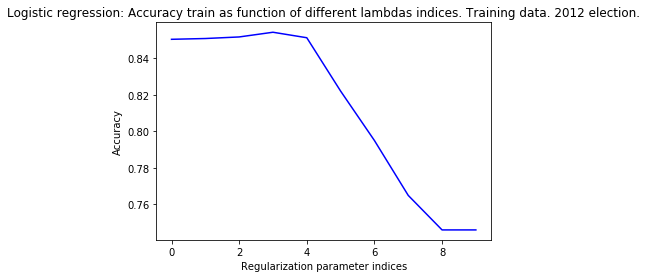
\includegraphics[width=0.7\textwidth]{pictures/results/Log_Reg_Train_2012}\label{fig:f3}}
    \hfill
  \subfloat[Test data 2012]{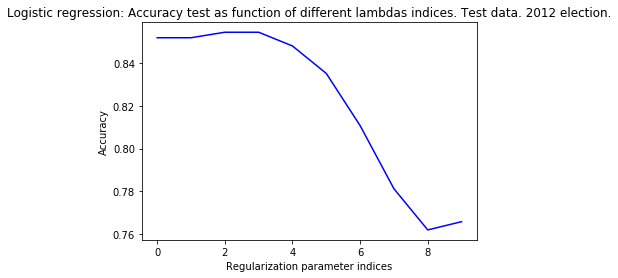
\includegraphics[width=0.7\textwidth]{pictures/results/Log_Reg_Test_2012}\label{fig:f4}}
    \hfill
  \subfloat[Test data 2016]{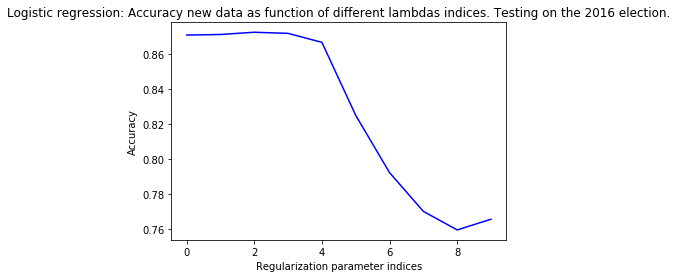
\includegraphics[width=0.7\textwidth]{pictures/results/Log_Reg_Test_2016}\label{fig:f4}}
   \caption{Accuracy graph}
\end{figure}
\newpage
\subsection{Linear SVM}
Scikit learn was also used to produce the SVM results below. The C's applied were values in the interval from 0.001 to 30. The accuracy stabilizes and peaks at C=3, index 1. The results are similar to logistic regression. This is not surprising, since they are both linear classifiers.  
\\
\par
\begin{figure}[H]
  \centering
  \subfloat[Train data 2012]{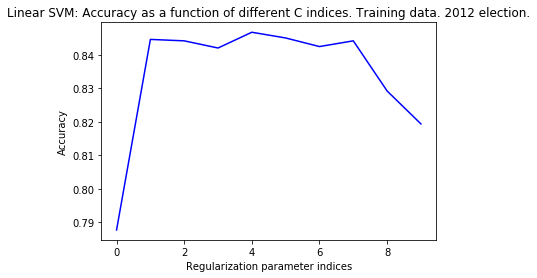
\includegraphics[width=0.7\textwidth]{pictures/results/Linear_SVM_Train_2012}\label{fig:f3}}
  \hfill
  \subfloat[Test data 2012]{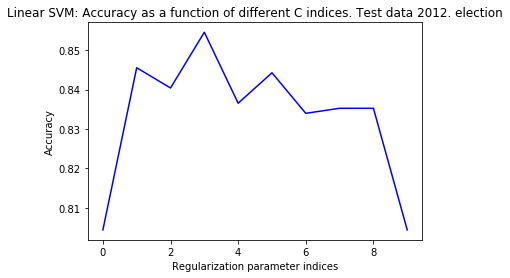
\includegraphics[width=0.7\textwidth]{pictures/results/Linear_SVM_Test_2012}\label{fig:f4}}
  \hfill
  \subfloat[Test data 2016]{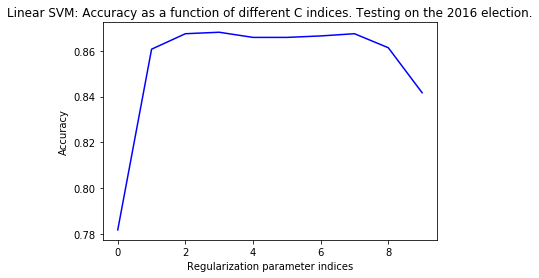
\includegraphics[width=0.7\textwidth]{pictures/results/Linear_SVM_Test_2016}\label{fig:f4}}
   \caption{Accuracy graph}
\end{figure}
\newpage
\subsection{Kernel SVM}
The C's values applied were the same as in linear SVM. The accuracy stabilizes and peaks at C=3, index 1. These results suggest that higher accuracy can be achieved by using the kernel trick.   
\\
\par
\begin{figure}[H]
  \centering
  \subfloat[Train data 2012]{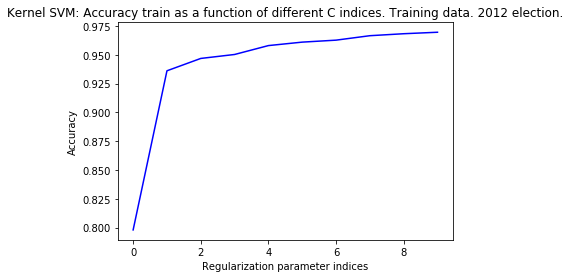
\includegraphics[width=0.7\textwidth]{pictures/results/Kernel_SVM_Train_2012}\label{fig:f3}}
  \hfill
  \subfloat[Test data 2012]{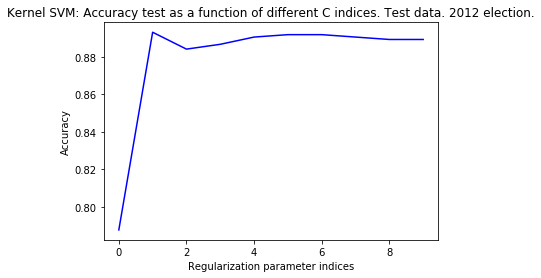
\includegraphics[width=0.7\textwidth]{pictures/results/Kernel_SVM_Test_2012}\label{fig:f4}}
  \hfill
  \subfloat[Test data 2016]{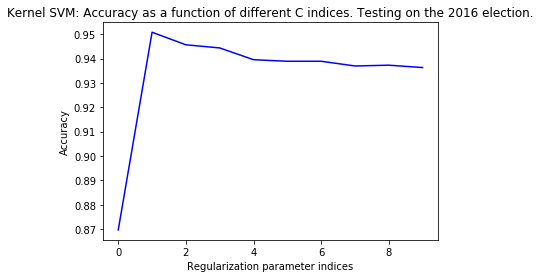
\includegraphics[width=0.7\textwidth]{pictures/results/Kernel_SVM_Test_2016}\label{fig:f4}}
   \caption{Accuracy graph}
\end{figure}
\newpage
\subsection{Neural network}
The optimal results were given by a layer set-up of [H,H,H,H,O] Were the activation functions for the hidden layers [H] were the Relu function, while the output layer [O] had Sigmoid as the activation function. The hidden layers were assigned 1000 neurons each. The optimization technique used is the stochastic gradient descent, SGD, with a batch size of 32 and 10 epochs. 
\\
\par 
\begin{figure}[H]
  \centering
  \subfloat[Train data 2012]{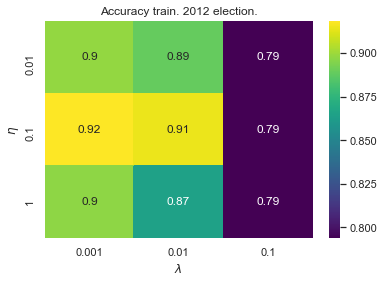
\includegraphics[width=0.5\textwidth]{pictures/results/NN_Train_2012}\label{fig:f3}}
  \hfill
  \subfloat[Test data 2012]{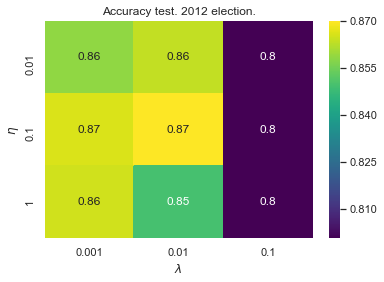
\includegraphics[width=0.5\textwidth]{pictures/results/NN_Test_2012}\label{fig:f4}}
  \hfill
  \subfloat[Test data 2016]{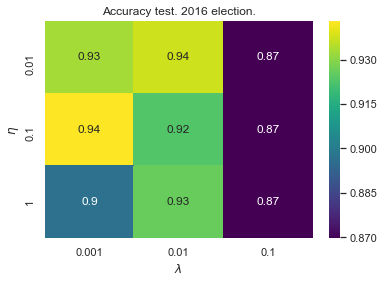
\includegraphics[width=0.5\textwidth]{pictures/results/NN_Test_2016}\label{fig:f4}}
  \caption{Accuracy heatmap}
\end{figure}
Validating neural network models with cross validation is computationally expensive. In order to avoid this, cross validation has been done with a low k, then less iterations. But a low k often gives worse and unreliable results, because the training data becomes significantly smaller. Cross validation results for all methods are found in the appendix [7].
\newpage
\subsection{Variable analysis}
Below present details regarding the variables impact on the results and on the flipped states between 2012 and 2016.
\begin{figure}[H]
\centering
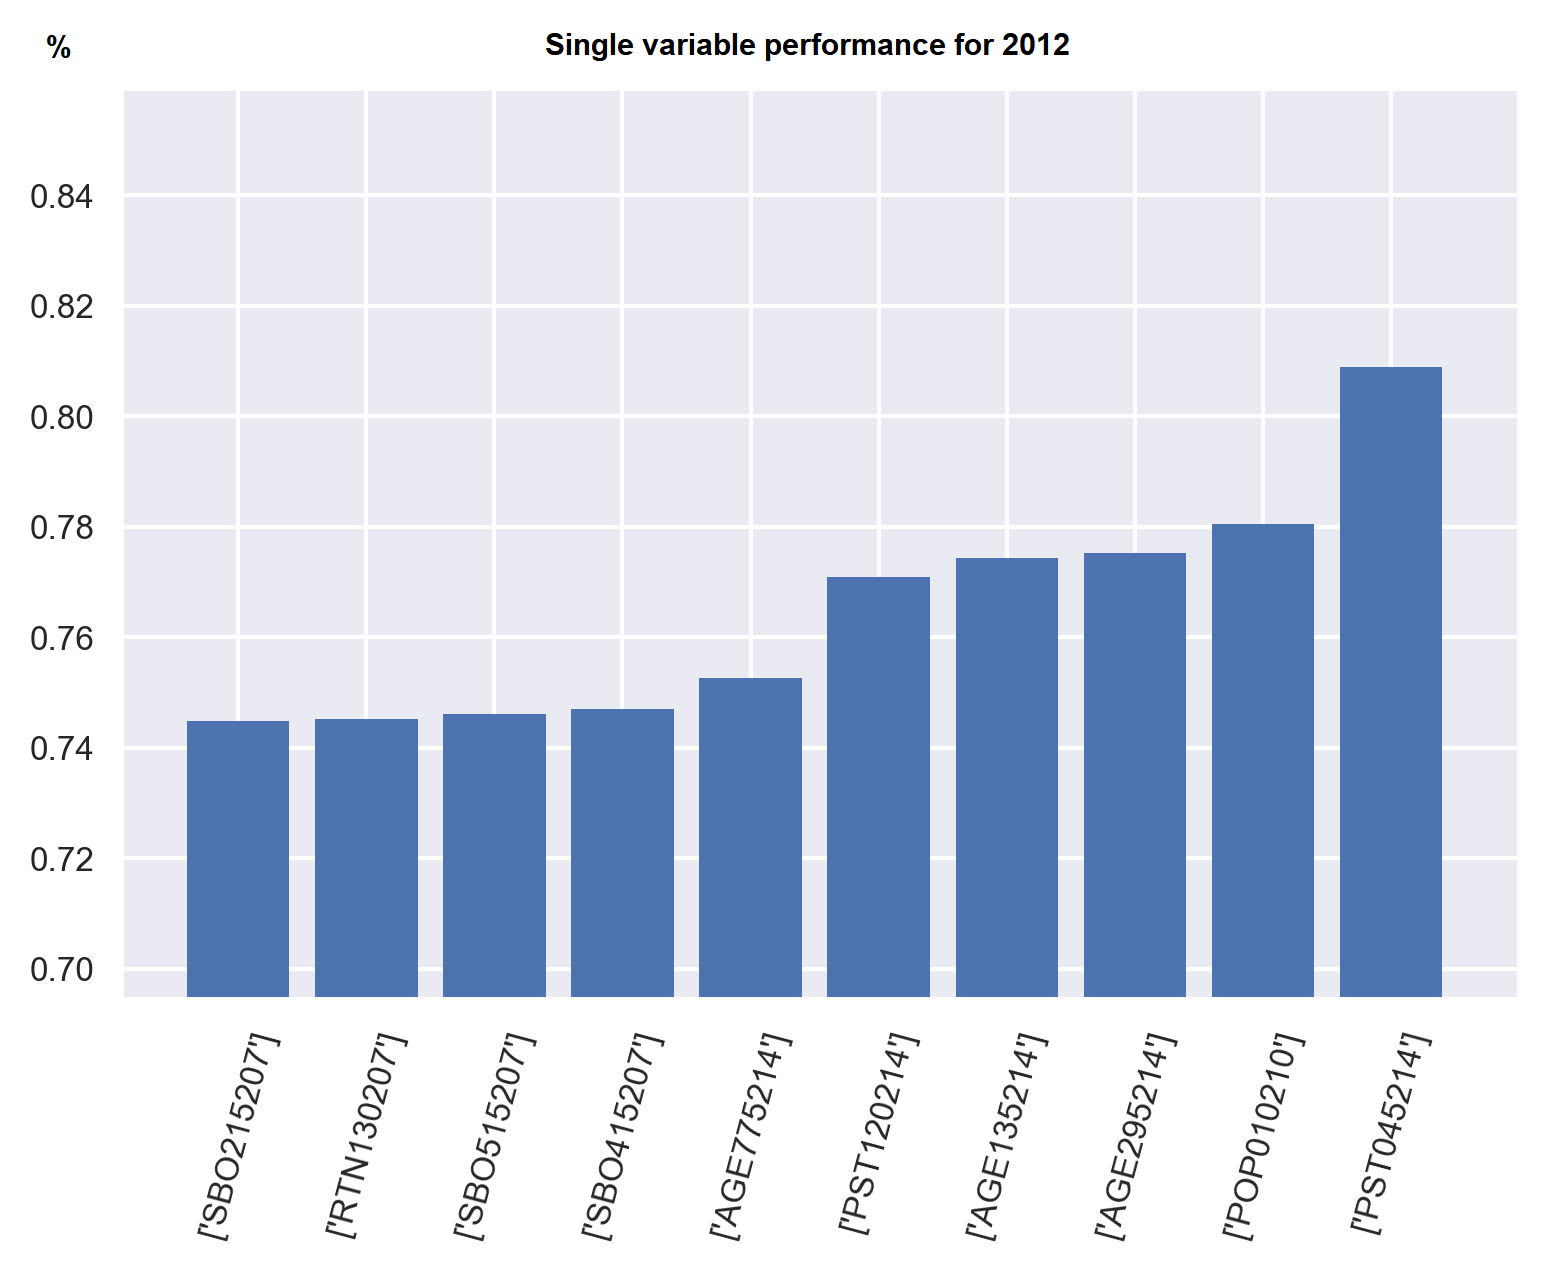
\includegraphics[scale=0.2]{pictures/results/max_12.png} 
\caption{Most explanatory variables with accuracy score}
\end{figure}
Graphics from test data against 2012. Calculated with SVM for gamma=0.00778, c=2, and a plain guess would be 78\%. This highlights the importance of the population and age variables as well as the one for firms. Further data can be found in the appendix [2].

\begin{figure}[H]
\centering
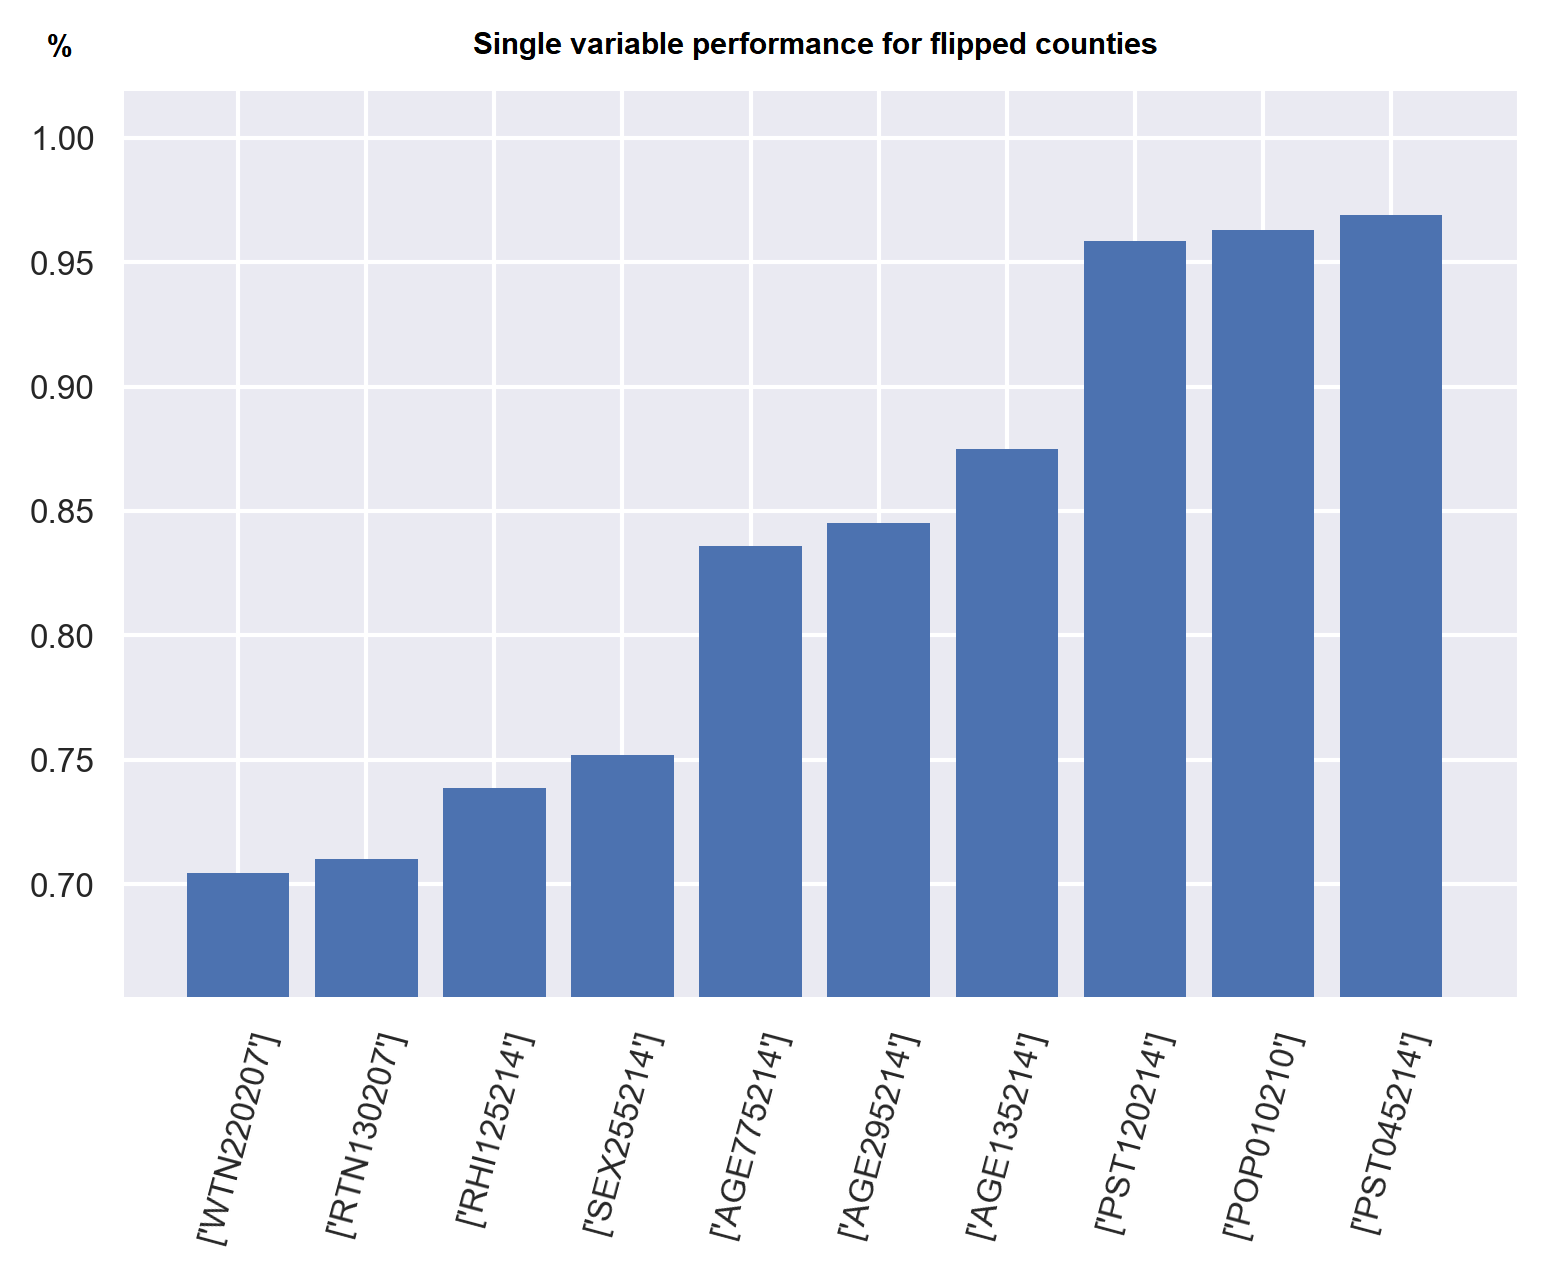
\includegraphics[scale=0.2]{pictures/results/max_flipp.png}
\caption{Most explanatory variables for flipped states with accuracy score}
\end{figure}
Graphics from test data against 2016. Calculated with SVM for gamma=0.00334, c=2, and a plain guess would be 95\%.

\begin{figure}[H]
\centering
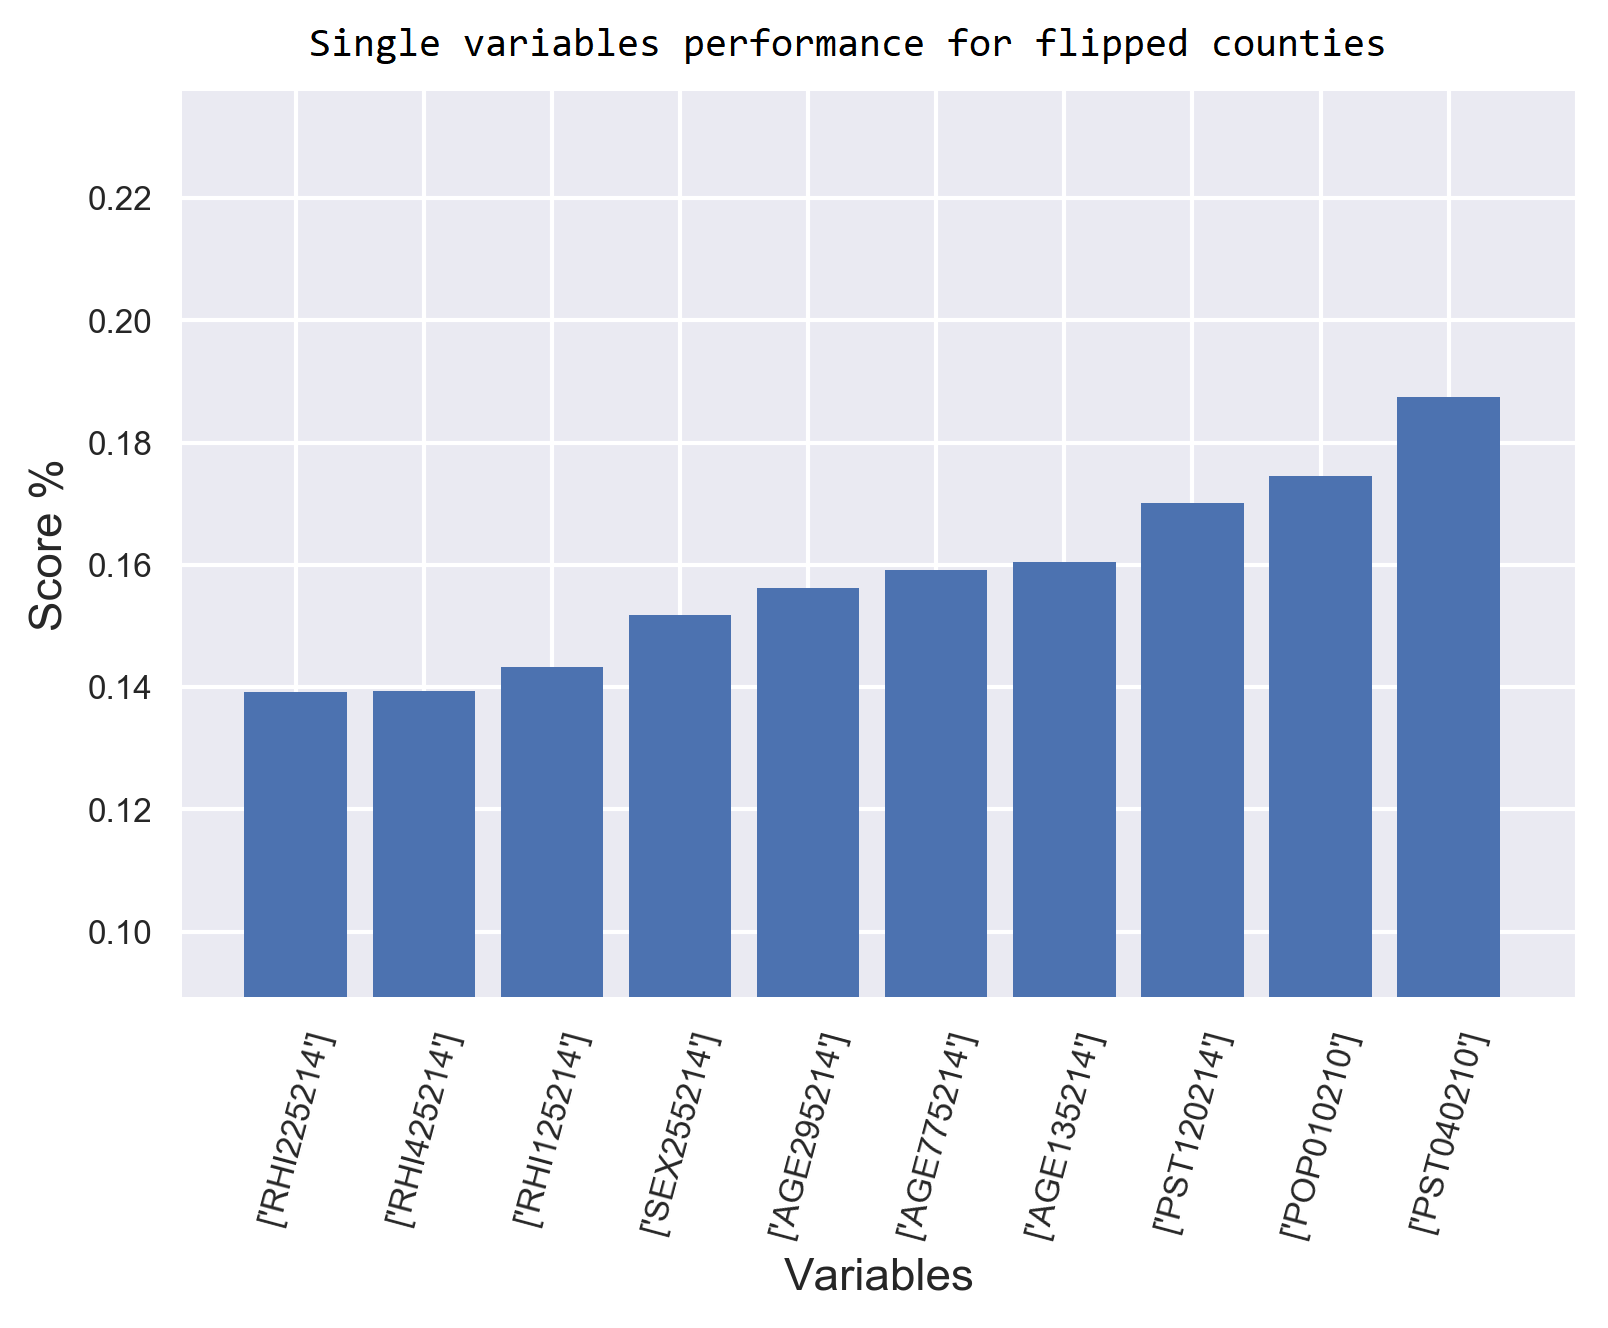
\includegraphics[scale=0.2]{pictures/results/f1_score.png} 
\caption{Most explanatory variables for flipped states with F1 score}
\end{figure}
Graphics from test data against 2016. Calculated with SVM for gamma=0.00778, c=2, and a plain guess would be 95\%. For the flipped case, age and population still have the most impact, but female percentage and white percentage are showing up as well.

\begin{figure}[H]
\centering
\subfloat[Age over 65]{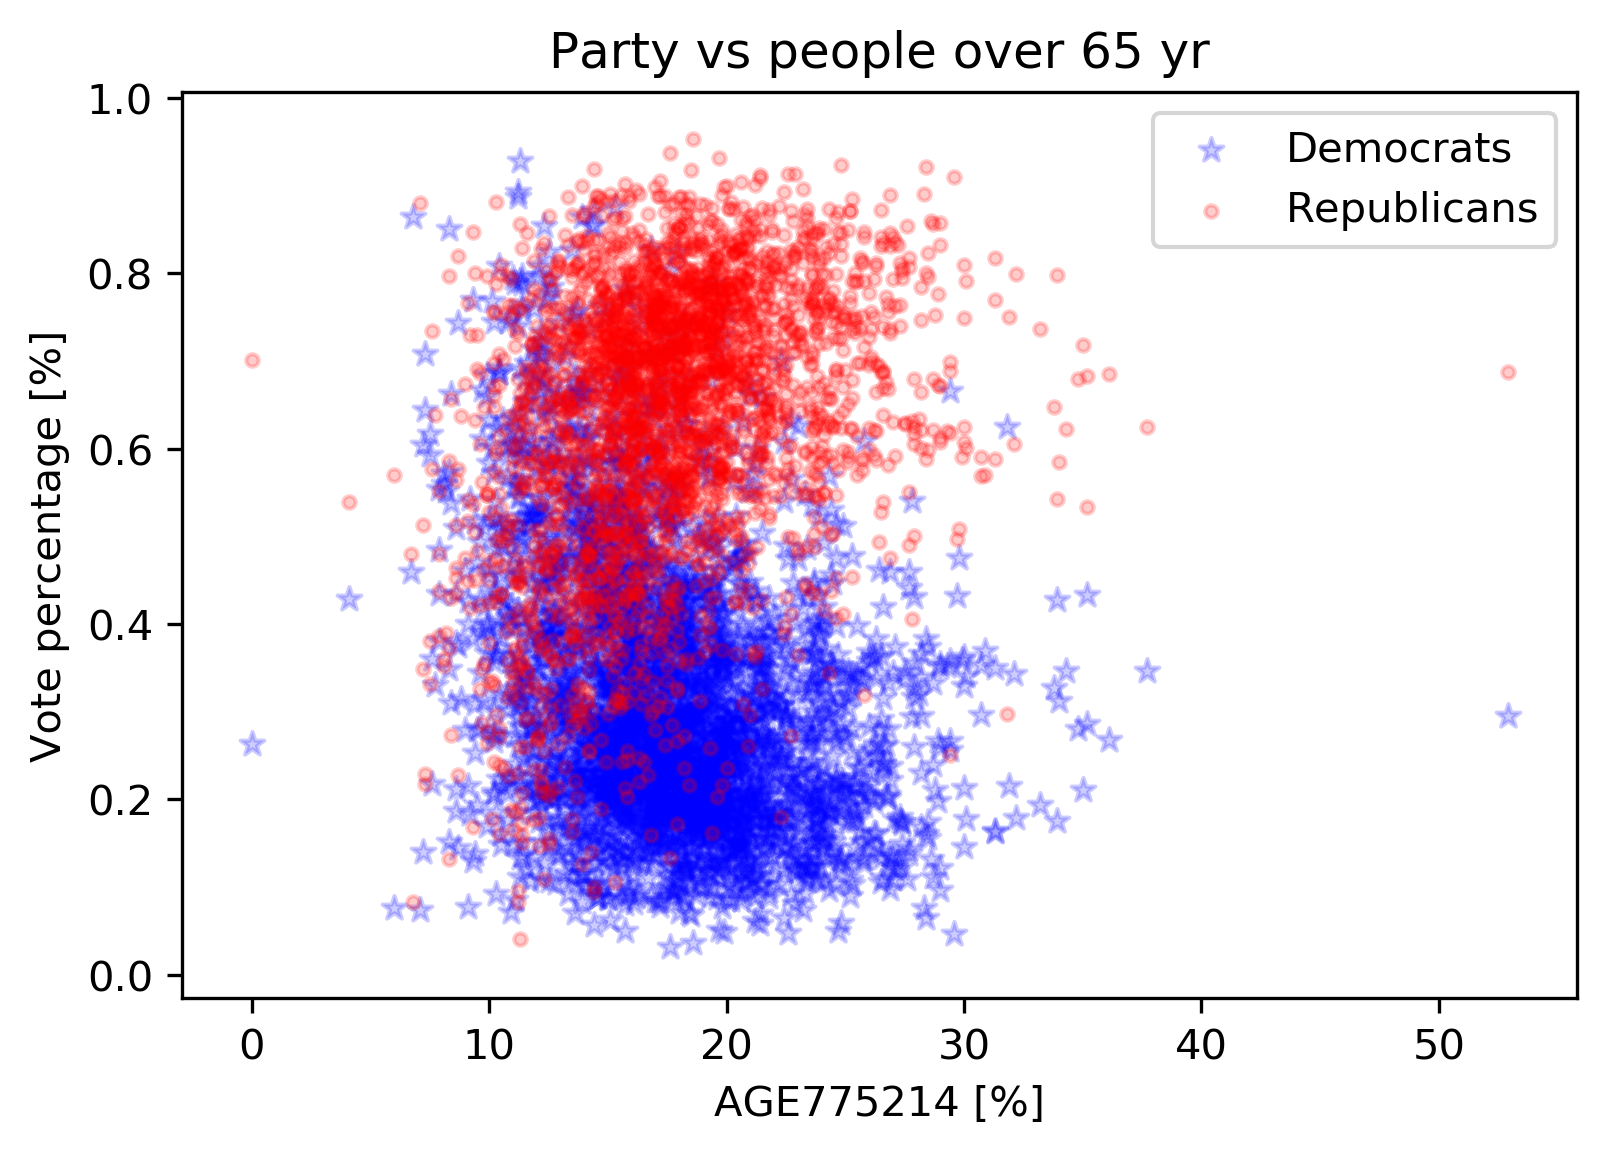
\includegraphics[width=0.5\textwidth]{pictures/results/dem_age.png}\label{fig:f3}}
\hfill
\subfloat[Population]{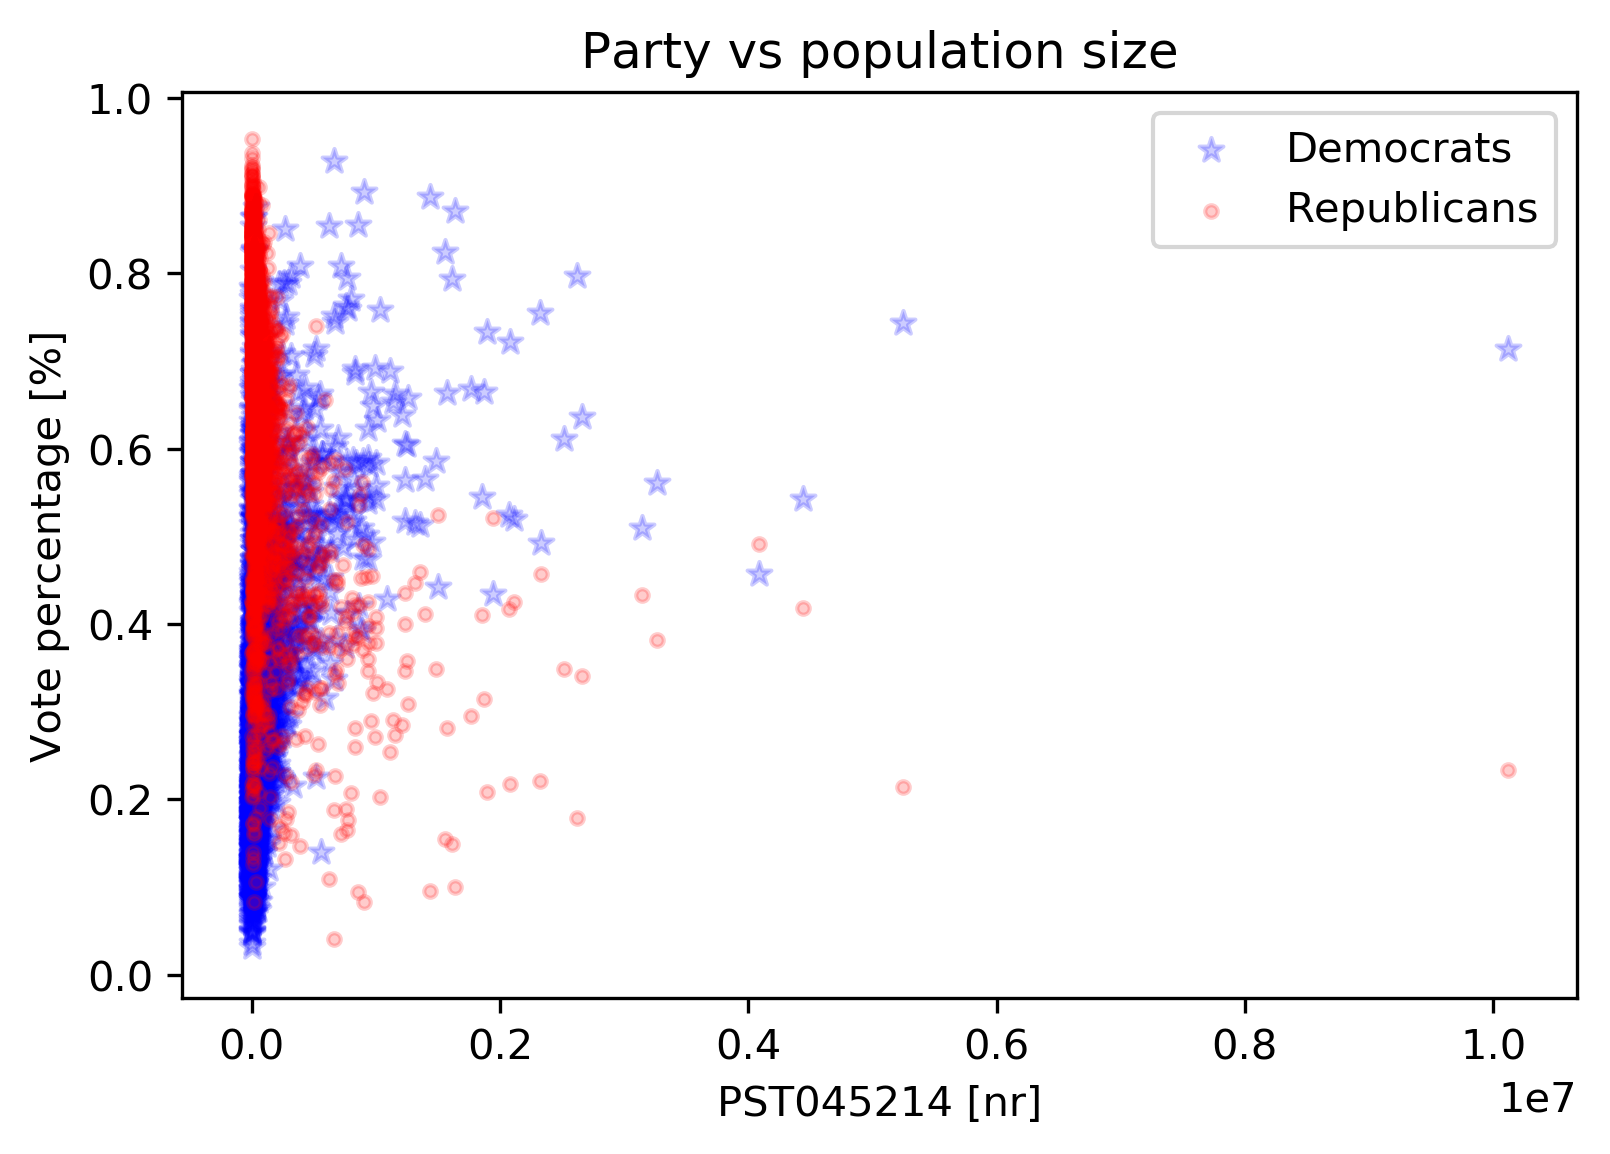
\includegraphics[width=0.5\textwidth]{pictures/results/dem_pop.png}\label{fig:f4}}
\caption{Scatter plot of important variables}
\end{figure}

An example that highlight the difference in political support is the variables age and population. One can see that for a county with 30\% percent old people, democrats are few. And with increased population, there is a decline in republicans.

\begin{figure}[H]
\centering
\subfloat[Females percentage]{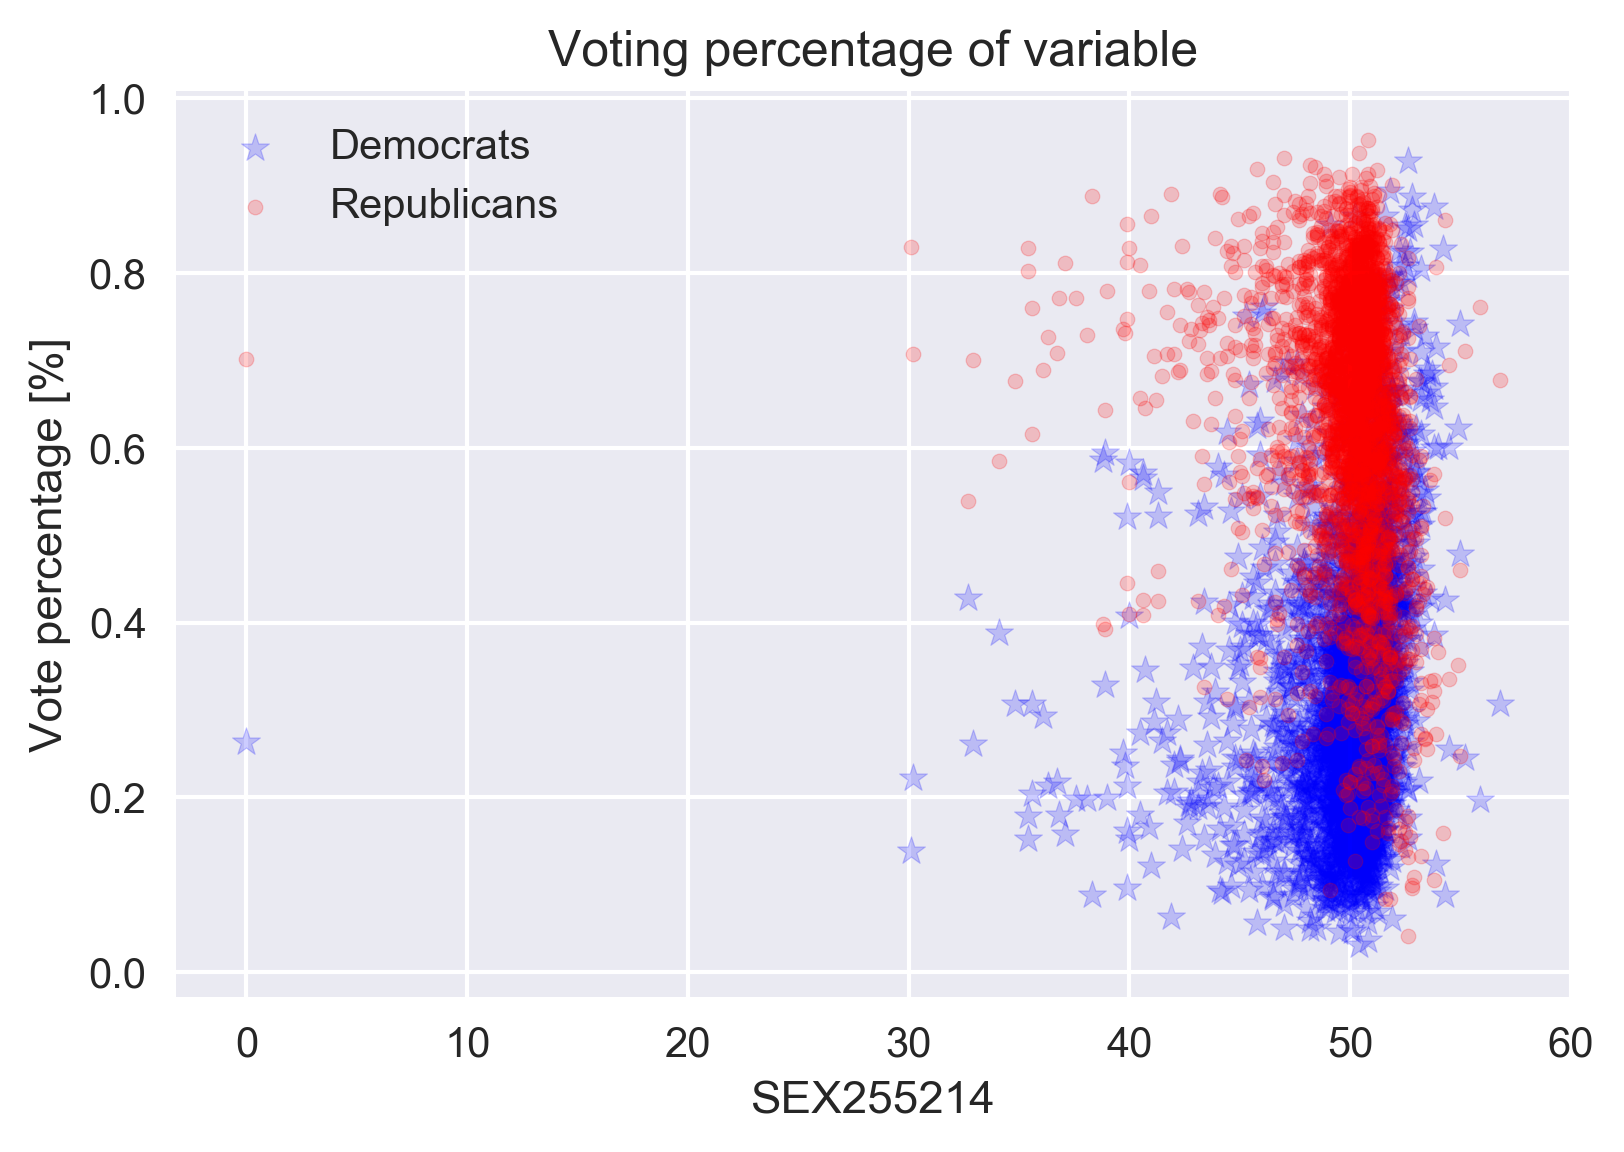
\includegraphics[width=0.5\textwidth]{pictures/results/dem_vs_females.png}\label{fig:f3}}
\hfill
\subfloat[White percentage]{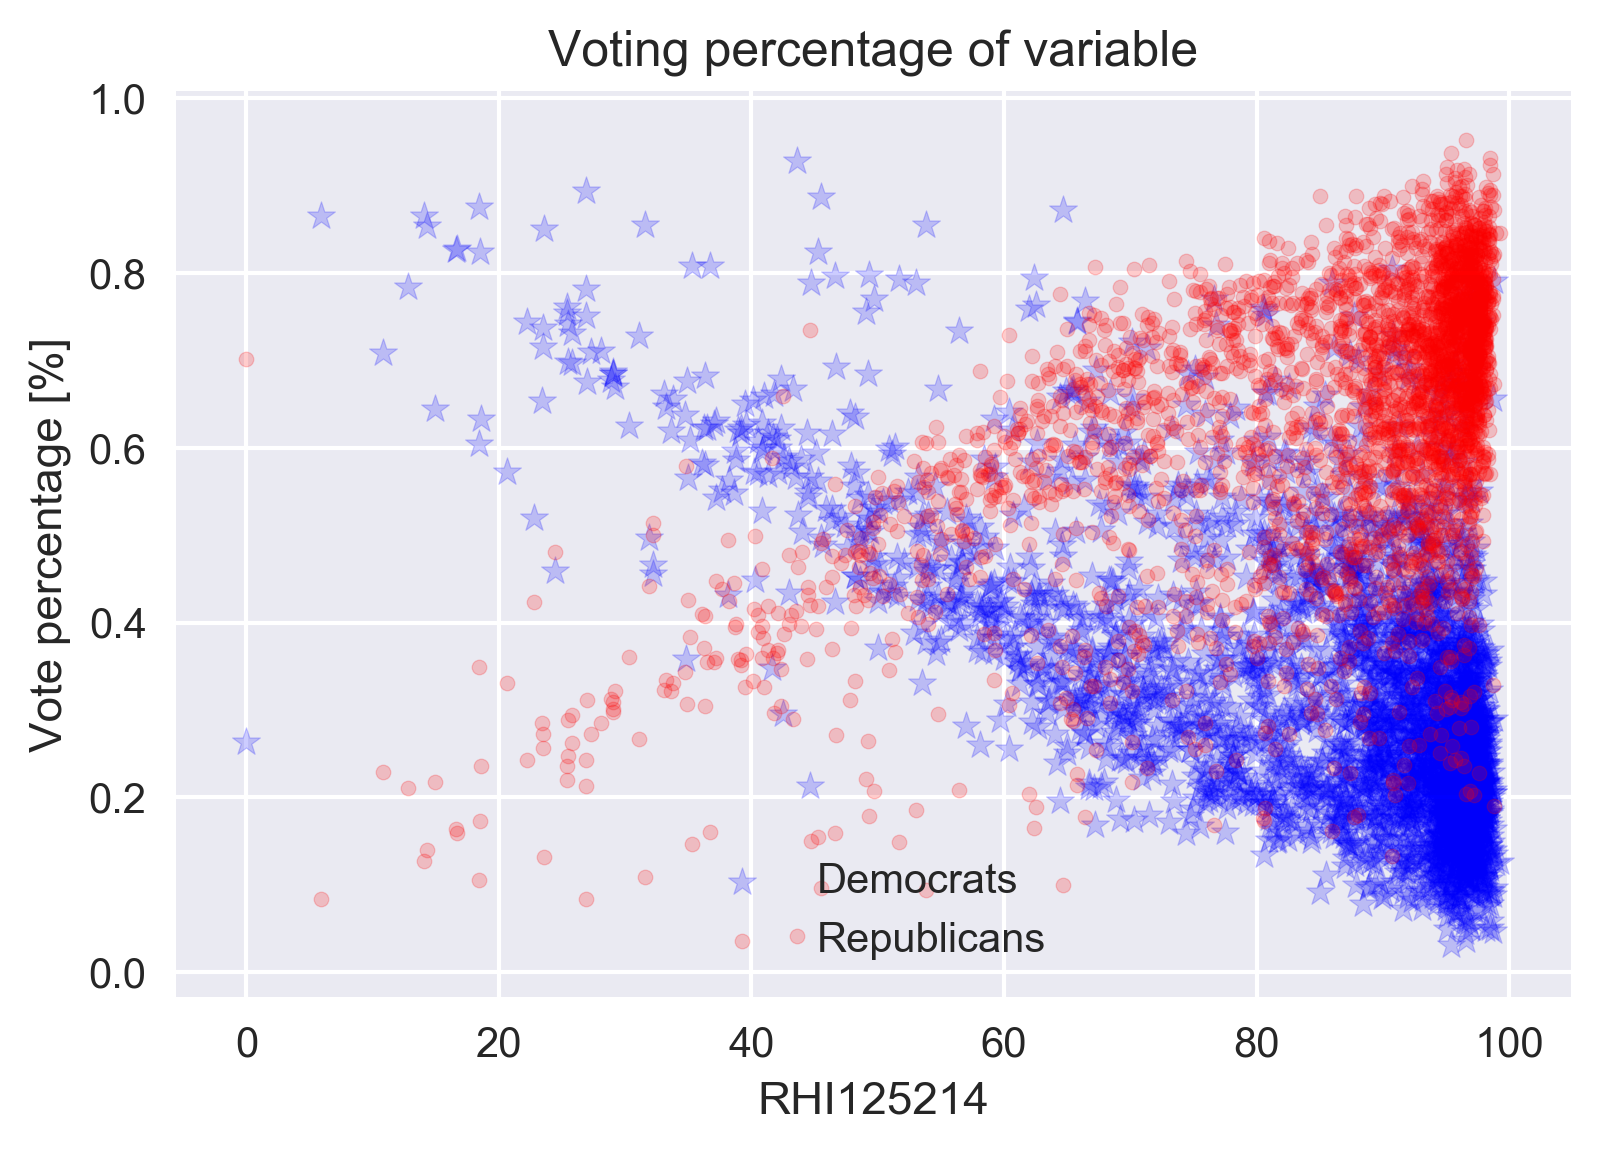
\includegraphics[width=0.5\textwidth]{pictures/results/dem_vs_white.png}\label{fig:f4}}
\caption{Scatter plot of important variables for flipped states}
\end{figure}
For the flipped counties the variables of white people percentage and female percentage stood out as slightly more important then the other variables, not considering the age and population. It is very clear how different these two groups vote.